% ---------------------------------------------------------------------- %

\documentclass[letterpaper,10pt]{article}



\pagestyle{empty}

\usepackage[table]{xcolor}
\usepackage{color, colortbl}
\usepackage{tabularx}
\usepackage{amssymb}
\usepackage{enumerate}

\definecolor{LightGray}{gray}{0.9}

\usepackage{amsmath}
\usepackage{amscd}
\usepackage{url}

\usepackage{graphicx}


\title{Standing Order for Data}
\author{Northwestern Seismology}
\date{\today}

\begin{document}
\maketitle


% ************************************************************* %
%                                                               %
%                       INSTALLING SOD                          %
%                                                               %
% ************************************************************* %

\section{Installation}

You can get SOD from here: \url{http://www.seis.sc.edu/sod/index.html}.
Once you have gotten the folder for SOD, put it somewhere where you won't touch it too much. What I did was put the SOD folder in my home directory, though other places are acceptable as well, as long as its not too easy to delete it by accident.

\begin{figure}[h!]
  \centering
  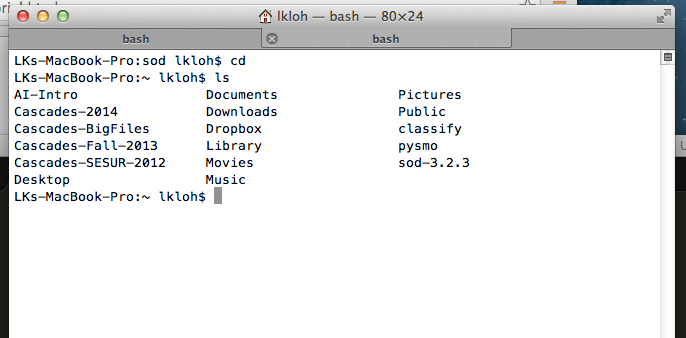
\includegraphics[width=0.5\textwidth]{images/sod_location}
  \caption{Path to sod bin}
  \label{fig:sod_location}
\end{figure}

Once you have it there, get the path to the sod folder's bin and put it in your path folder. 


\begin{figure}[h!]
  \centering
  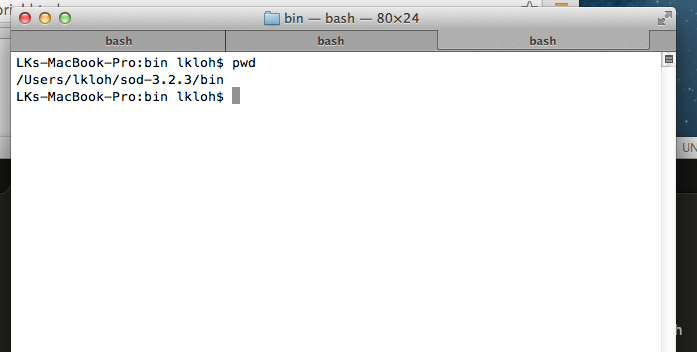
\includegraphics[width=0.5\textwidth]{images/path_to_sod_bin}
  \caption{Path to sod bin}
  \label{fig:path_to_sod_bin}
\end{figure}

Inside my home directory's bash profile (you get the by typing \verb"cd"), you put the path to \verb"sod-3.2.3/bin" by adding in either the \verb"bash" or \verb"bash_profile" or \verb"profile" files: 
 
\begin{figure}[h!]
  \centering
  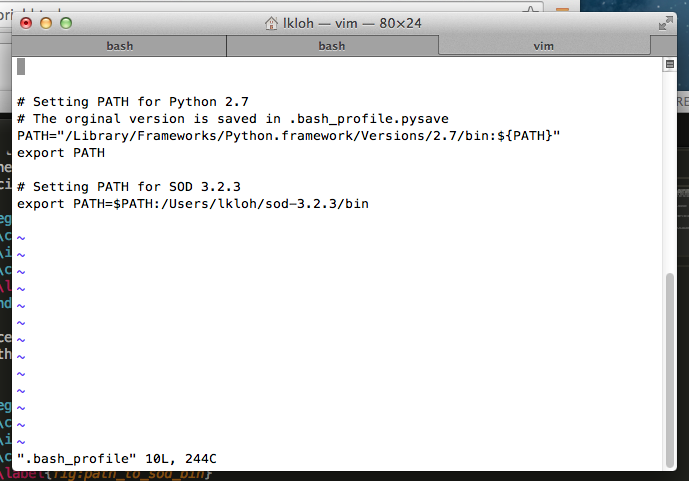
\includegraphics[width=0.5\textwidth]{images/home_bash_profile}
  \caption{bash profile}
  \label{fig:home_bash_profile}
\end{figure}

To check if SOD has been installed properly, close the terminal, restart it, and type \verb"sod". If that works, we should see something like this: 

\begin{figure}[h!]
  \centering
  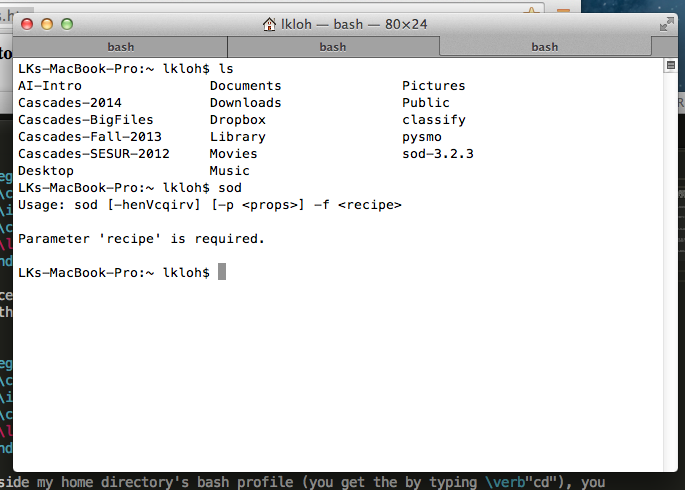
\includegraphics[width=0.5\textwidth]{images/sod_installed_query}
  \caption{Is SOD installed?}
  \label{fig:sod_installed_query}
\end{figure}

% ************************************************************* %
%                                                               %
%                       INSTALLING SOD                          %
%                                                               %
% ************************************************************* %

% ************************************************************* %
%                                                               %
%                    DOWNLOAD DATA WITH SOD                     %
%                                                               %
% ************************************************************* %

\section{Downloading Data with SOD}

\textsc{By Trevor Bollman}

\begin{enumerate}
  \item Create a sod recipe and place it in the folder that you would like the data to download to.
        \begin{verbatim}
          sod -f <recipename>.xml
        \end{verbatim}
  \item Run \verb"sodcut.sh" to cut the seismogram around phase wanted
        \begin{itemize}
          \item check model within \verb"cutevseis.sh"
          \item run using \verb"sodcut.sh <name>"
          \item watch sdir = processed seismograms
          \item Run over the entire downloaded directory (the files sod downloaded)
        \end{itemize}
  \item Run \verb"sodpkl.sh" (converts \verb".sac" files to python pickles)
        \begin{enumerate}
          \item run using \verb"sodpkl.sh [options] <directory>""
          \item output will automatically be zipped
          \item run in DATA directory
        \end{enumerate}
  \item run \verb"ttpick.py" (does travel time picking with plotting)
        \begin{enumerate}
          \item can use \verb"iccs.py" but it does not have plotting capabilities
          \item run using \verb"ttpick.py [options] <pkl.gz file>"
          \item do this one event at a time
          \item use \verb"sacp2" to look at the stacking of the seismograms
          \item you can sort the seismograms using the \verb"–s" flag
        \end{enumerate}
  \item run \verb"getsta.py" (creates a \verb"loc.sta" file)
        \begin{verbatim}
          getsta.py [options] <pkl.gz files>
        \end{verbatim}
  \item Run EITHER of these: 
        \begin{enumerate}
          \item \begin{itemize}
                  \item run \verb"mccc2delay.py" (converts mccc delays to actual delays)
                        \begin{verbatim}
                          mccc2delay.py [option] <.mcp files>
                        \end{verbatim}
                  \item run \verb"getdelay.py" (creates a delay file)
                        \begin{verbatim}
                          getdelay.py [options] <*.px>
                        \end{verbatim}
                  \item Can possibly use \verb"doplotsta.sh", plots all of the events and their station delays
                \end{itemize}
          \item Run \verb"evmcdelay.sh"
        \end{enumerate}
  \item \verb"ttcheck.py" to compare the delay times of the p and s waves. Should form a nice cloud with the mean value in line with the cloud.
  \item If you need to remove a station from an event you can use \verb"pklsel.py"
        \begin{itemize}
          \item Run using \verb"pklsel.py [pkl file] –d [stnm]" to remove one station
          \item Only works for one event at a time
        \end{itemize}
  \item If you need to filter the data to be able to pick use \verb"evsacbp.sh"
        \begin{itemize}
          \item run using \verb"evsacbp.sh [pkl file] bp1 bp2"
          \item Automatically uses two corners
          \item run in the whole downloaded directory (the one with the sac directory)
        \end{itemize}
\end{enumerate}



% ************************************************************* %
%                                                               %
%                    DOWNLOAD DATA WITH SOD                     %
%                                                               %
% ************************************************************* %


% ------------------------------------------------------------------------- %


\end{document}

% --------------------------------- END --------------------------------- %
